\documentclass[oneside]{article}

% ---------------------------------------------
% Importing packages
% ---------------------------------------------

% Encoding and font
\usepackage[utf8]{inputenc}
\usepackage{tgcursor}
\usepackage{hyperref}
\usepackage{wrapfig}

% Different colors
\usepackage{xcolor}
\usepackage{color}
\definecolor{bluepoli}{cmyk}{0.4,0.1,0,0.4}

% Math
\usepackage{amsmath}
\usepackage{amsthm}

% Chemistry
\usepackage[version=4]{mhchem}

% Images
\usepackage{graphicx}
% \graphicspath{ {./Figures/} }

% Margins
\usepackage[a4paper, top=2cm, left=2.5cm, right=2.5cm, bottom=2cm]{geometry}

% Fancy header and footer
\usepackage{fancyhdr}
\pagestyle{fancy}
\fancyhf{}
\rhead{Calcoli di Processo dell'Ingegneria Chimica}
\lhead{Practical Session 5}
\rfoot{Page \thepage}
\lfoot{Academic Year 2024-2025}


\usepackage{amsthm}
\usepackage{tcolorbox}
\tcbuselibrary{most}
\tcolorboxenvironment{proof}{% `proof' from `amsthm'
   blanker,
   breakable,
   left=5mm,
   before skip=10pt,
   after skip=10pt,
   borderline west={1mm}{0pt}{bluepoli}
}

% ---------------------------------------------
% Title
% ---------------------------------------------

\title{Practical Session 6}
\author{Timoteo Dinelli\footnote{timoteo.dinelli@polimi.it}, Marco Mehl\footnote{marco.mehl@polimi.it}}
\date{15\textsuperscript{th} of November 2024}

% ---------------------------------------------
% Begin of the document
% ---------------------------------------------

\begin{document}
\maketitle

\section{``La media mobile''}
In statistica, la media mobile è uno strumento utilizzato per l'analisi di serie
storiche. In particolare, le medie mobili vengono ampiamente utilizzate nell'analisi
tecnica delle fluttuazioni delle quotazioni di un bene. La media mobile attribuisce ad ogni valore della
variabile indipendente (in genere il tempo) un valore della funzione pari alla media di
tutti i valori precedenti a quel momento per un certo intervallo ($n$ elementi) riducendo
il "rumore" nei dati e mettendo in evidenza dei possibili trend.
Quindi, data la seguente serie di coppie $(x, \:y)$:
\begin{table}[h!]
   \centering
   \begin{tabular}{c | c}
      x & y \\ \hline
      0 & 1 \\
      1 & 2 \\
      2 & 3 \\
      3 & 4 \\
      4 & 5 \\ \hline
   \end{tabular}
\end{table}
Una media mobile semplice di ordine \textbf{2} partirebbe dalla seconda coppia e calcolerebbe il
valore associato al punto $x(2) = 1$ come la media di $y(2) = 2$ e $y(1) = 1$, mentre al punto
successivo $x(3) = 2$ verrebbe associato il valore medio tra $y(3) = 3$ e $y(2) = 2$. Otterremmo
quindi una serie di coppie $(x_{mm}, \: y_{mm})$ come la seguente:
\begin{table}[h!]
   \centering
   \begin{tabular}{c | c}
      x\textsubscript{mm} & y\textsubscript{mm} \\ \hline
      1 & 1.5 \\
      2 & 2.5 \\
      3 & 3.5 \\
      4 & 4.5 \\ \hline
   \end{tabular}
\end{table}
Si noti come la serie mm inizi in ritardo rispetto ai dati originali. Si chiede di
scrivere una funzione che prenda come input una coppia di vettori $(x, \: y)$ di
lunghezza $l$ e restituisca una coppia di vettori $(x_{mm}, \: y_{mm})$ di lunghezza
$l-n+1$ dove $n$ è l'ordine (il numero di elementi da mediare) della media mobile.

\section{``Conversione di ammoniaca \ce{NH3}''}
Si chiede di diagrammare la conversione del processo di produzione dell' ammoniaca
rispetto alla temperatura [600K 900K]  sapendo che la reazione è controllata
dall’equilibrio.

La reazione di interesse è: \ce{N2 + 3 H2 -> 2 NH3}.

Ricordando le seguenti relazioni:

\begin{align}
   K_P (T)  &= \frac{y_{NH_3}^2}{y_{H_2}^{3} y_{N_2}} \frac{1}{P^2}, \; y_{NH_3} =
   \frac{n_{NH_3}}{n_{tot}}, \; y_{H_2}  = \frac{n_{H_2}}{n_{tot}}, \; y_{N_2}  =
   \frac{n_{N_2}}{n_{tot}} \\
   n_{tot} &= 4 - 2\lambda, \; n_{NH_3} = 2\lambda, \; n_{H_2} = 3 - 3\lambda, \; n_{N_2}
   = 1 - \lambda.
\end{align}

Sapendo che la composizione di equilibrio può essere calcolata dall' equazione 1, e che
le frazioni molari in fase gas $y$ delle specie coinvolte nella reazione possono essere
scritte in funzione di una variabile $\lambda$ detta grado di avanzamento della reazione
basata sulla conversione dell' azoto come indicato nelle espressioni indicate come nell'
equazione 2, si chiede di mappare il valore di $\lambda$ nello spazio delle temperature
$T_i$ e delle pressioni $P_i$ utilizzando la funzione {\it contourf} nello spazio
compreso tra $600\:K$ a $900\:K$ e da $50\:atm$ a $600\:atm$. Si scriva poi una funzione
che calcoli il valore della costante di equilibrio {\it k} in funzione della temperatura.

\subsection*{Dati}
\begin{itemize}
   \item $dH = -22 \: kcal/mol$.
   \item $dS = -47.35 \: cal/mol/K$.
   \item Si ricorda che valgono le seguenti relazioni termodinamiche: $dG_{0} = dH - T \:
      dS$, $Kp = e^{\left( -\frac{dG0}{RT} \right)}$.
\end{itemize}

\section{``Stuntman''}

\begin{wrapfigure}{r}{0.3\textwidth}
   \centering
   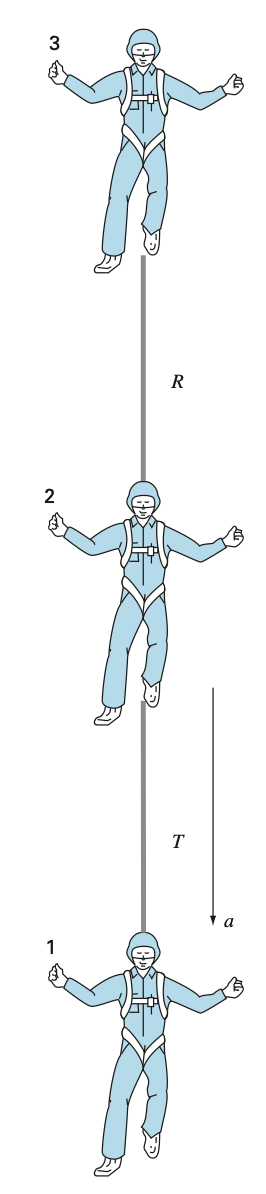
\includegraphics[width=0.25\textwidth]{stuntman.png}
\end{wrapfigure}

Sul set di un film di azione 3 stuntman cercano di capire come esercitarsi in sicurezza
per una scena che prevede la caduta da un'altezza di $15 \: m$. I 3 sono collegati tra
loro da 2 corde, che vengono considerate senza peso, mentre sono in caduta libera. La
velocità di un corpo in caduta libera può essere calcolata utilizzando l'equazione del
moto rettilineo uniformemente accelerato $v^2 = v_{init}^2 + 2a(s - s_0)$ dove $v$ é la
velocità, $v_{init}$ la velcità iniziale, $a$ l'accelerazione e $s$ lo spostamento. In
caduta libera, un corpo è soggetto all'accelerazione gravitazionale, che è
approssimativamente di $9.81 \: \frac{m}{s^2}$ sulla superficie terrestre. Le masse degli
stuntman sono $m_1 = 70 \: kg$, $m_2 = 60 \: kg$, $m_3 = 40 \: kg$. Prima di effettuare
l' esercitazione si vuole avere una stima della tensione che le 2 corde subiranno
assumendo che la velocità di caduta dei 3 collegati sia pari a quella di caduta libera.
Per semplicità si applica la seconda legge di Newton: $m \: a = \sum_{i=0}^{n}F_i$ dove
$m$ è la massa, $a$ l'accelerazione e $F_i$ le singole forze agenti sul corpo, tra le
quali è necessario ora considerare anche la forza di resistenza esercitata dall'aria come
$F_{drug} = c_{drug} v_{free fall}$, dove $v_{free fall} = \sqrt{2gh}$. I coefficienti
dei singoli stuntman sono rispettivamente $c_1 = 10 \frac{kg}{s}$, $c_2 = 14
\frac{kg}{s}$, $c_3 = 17 \frac{kg}{s}$. Si chiede quindi di calcolare la tensione in ogni
corda e l'accelerazione del team.

\end{document}
